
\section{Quantum Mechanics}
Quantum Mechanics(QM) was formulated to overcome some important limitations in classical mechanics; the inability of Newtonian mechanics to explain radiation properly and to make an appropriate prediction of phenomena in a microscopic scale.\cite{zettili2009} \acrshort{QM} is the best known theoretical foundation for describing our known universe. In \acrshort{QM}, a Hilbert space\footnote{Hilbert space is an infinite-dimensional inner product vector space. We use a finite-dimensional Hilbert space for our study} called state space is associated with any physical system and is denoted by its state vector $\ket{\Psi}$ \footnote{$\ket{.}$ is a Dirac's ket} \cite{Nielsen2002}(Neilsen and Cheung,2005). The state vector $\Psi(x,y,z,t)$, a function of space and time,  gives all the information about the system. Although, $\Psi$ alone does not have much meaning by itself. The only quantity having physical meaning is the square of its magnitude $P = {\mid\Psi\mid}^{2} = \braket{\Psi|\Psi}$, which gives the probability density of the state. \cite{murugeshan}(Murugeshan, 2015). Here every dynamical variable in classical mechanics or observable like position, momentum, energy, is an operator. Each operator is unitary matrices which on acting upon state vector $\ket{\Psi}$ gives the possible result as their eigenvalues. Since the observable are operators in \acrshort{QM}, the act of observation affects the state of the system. Operation by an arbitrary operator A is denoted by $\braket{\Psi|A|\Psi}$\footnote{$\braket{\Psi|A|\Psi}$ means the inner product of $\ket{\Psi}$ and $A\ket{\Psi}$}.

\section{Quantum Computing}
Feynman, in 1981, talked about a possibility of a computer that will do exact simulation same as by nature.\cite{feynman1999} It has been theoretically and experimentally proven that nature follows the rules of Quantum mechanics at microscopic levels. He added an example of polarization of photon(a two-state system) to make his point that "quantum mechanics can't seem to be imitable by a local classical computer".\cite{feynman1999}(Feynman1999, 485)  Classical computer uses classical physics which are deterministic in nature while quantum mechanics is probabilistic and is reversible. Another significant issue for classical mechanics is that it uses Boolean algebra, which states distributive property. But quantum mechanics does not necessarily follow the property\cite{calabrese2005}. "A Quantum computer is a device that leverages certain properties described by quantum mechanics to perform computation." \cite{Hidary} (Hidary, 2019, 3) Quantum computers(\acrshort{QC}) uses properties like entanglement, superposition, and reversibility.

Different algorithms have been designed in the field whose equivalence in classical computing performs rather slow and lacks efficiency in performance. Shor's prime number factoring algorithm, Grover's search algorithm are some notable examples. However, no efficient and functional quantum computer has been built yet. Physicists and engineers have been using different architectures to realize a working efficient \acrshort{QC}. Superconducting qubits, trapped ion qubits, Nuclear magnetic resonance, silicon-based spin qubit are some physical systems that currently realize quantum computation, on a small scale.\cite{Hidary} Regardless of that, studying and discussing quantum algorithms does not necessarily require a workable quantum computer and not even detailed knowledge about the physics of quantum computers.\cite{Cheung}

The first experimental implementation of Shor's algorithm on a quantum computer was performed by a group at IBM in 2001 using nuclear magnetic resonance to factor an integer 15. \cite{vandersypen2001experimental} The largest integer ever factored using  Shor's algorithm is 21, performed in 2012 by scientists at the University of Bristol.\cite{martin2012experimental}
Classical computers use bits as the basic unit of information. A bit takes one of the two states: 0 or 1. Qubit is similar to the classical bit, however, the main significant difference is that qubits may be in the superposition of both the states $\ket{0}$ and $\ket{1}$. A system described  by state vector $\ket{\Psi}$ is said to be in superposition of state $\ket{0}$ and $\ket{1}$ if $\ket{\Psi}$ is the linear combination of $\ket{0}$ and $\ket{1}$, written as \begin{equation}\ket{\Psi} = \alpha\ket{0} + \beta\ket{1}\label{eq: 2.1}\end{equation}
where $\alpha$ and $\beta$ are complex coefficients called amplitudes of each states following normalization rule: ${|\alpha|}^{2} + {|\beta|}^{2} = 1$. "A qubit can exist in a continuum of states between $\ket{0}$ and $\ket{1}$ - until it is observed."(Neilsen and Chuang, 2002, pg. 3)\cite{Nielsen2002} As stated earlier: the act of observation affects the state of the system, measurement of the state vector $\ket{\Psi}$ collapse superposition of the state to one of the two basis states $\ket{0}$ or $\ket{1}$. The square of their amplitude gives the probability of obtaining each state upon measurement. However, direct measurement does not give any information about $\alpha$ or $\beta$. They are obtained by measuring the quantum state of the state vector and other similar state vectors resembling it. The accuracy of measuring $\alpha$ and $\beta$ is based on the number of measurements made or numbers of similar quantum states measured.



A single qubit represented as $\ket{\Psi} = \alpha\ket{0} + \beta\ket{1}$(also written as $\begin{pmatrix}\alpha \\ \beta \end{pmatrix}$) is a two dimensional unit vector in a  complex vector space $\mathbb{C}^{2}$ spanned by basis vectors $\ket{0} = \begin{pmatrix} 1 \\ 0\end{pmatrix}$  and $\ket{1} = \begin{pmatrix} 0 \\ 1\end{pmatrix}$ and a two qubit system would be represented by a four dimensional unit vector spanned by basis states $\ket{00}$, $\ket{01}$,$\ket{10}$ and $\ket{11}$. Similarly, a n qubit system would be spanned by $2^{n}$ different basis states from 0 to $2^{n}-1$ binary equivalent, written as 
\begin{equation}
\ket{\Psi} = \sum_{m=0}^{2^{n}-1} a_{m}\ket{m}\label{eq:2.2}
\end{equation},
where $\ket{m} = \ket{x_{1}x_{2}...x_{m-1}x_{m}}$ has the binary representation such that $m = 2^{m-1}x_{1} + 2^{m-2}x_{2} + ... + 2^{1}x_{m-1} + 2^{0}x_{m}$,  $x_{i}\in \{0,1\}$. So a n qubit system represents and manipulates $2^{n}$ classical equivalent states.  This gives a slight idea about the supremacy \acrshort{QC} has over classical computers. A single qubit lie in a $\mathbb{C}^{2}$ space and similarly, a n qubit system lies in a space with the dimension equal to the tensor product of each qubits, \begin{equation} \mathbb{C}^{2} \otimes \mathbb{C}^{2} \otimes ... \otimes \mathbb{C}^{2} = ({\mathbb{C}^{2}})^{\otimes n} =  \mathbb{C}^{2^{n}} \end{equation}.\cite{Cheung} Hence, each state $\ket{m}$ can be written as the tensor product: $\ket{m}=\ket{x_1}\otimes\ket{x_2}\otimes...\ket{x_n}$.
\\
Another useful and intuitive way of representing a state of the qubit is by using state vector in the Bloch sphere. The state vector is given by equation: \begin{equation}
    \ket{\Psi}= e^{i\gamma}(\cos\frac{\theta}{2}\ket{0} + e^{i\phi}\sin\frac{\theta}{2}\ket{1})
    \label{eq: 2.4}
\end{equation}
where $\theta$, $\phi$ and $\gamma$ are real numbers. Different values of $\theta$ and $\phi$ sweeps each point of the sphere. Each point on the Bloch sphere can be a possible state of a qubit. Most of the operations on qubits can be visualized or interpreted as the rotation of the state vector in the Bloch sphere.

\begin{figure}
    \centering
    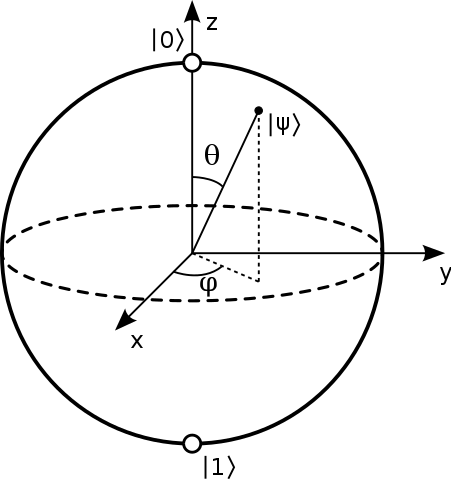
\includegraphics[width= 5cm, height=5.32cm] {blochsphere1.png}
    \caption{Qubit representation in a Bloch sphere}
\end{figure}
    
    

Any two-level quantum system can be realized as a physical qubit, for instance, the ground state and excited state of an atom or two spin states of a 1/2 spin electron or horizontal and vertical polarization of the photon.\cite{DiVincenzo} But qubits are delicate things; they lose their coherence rapidly and their state is affected by small interaction. This is a reason why a general-purpose quantum computer is hard and challenging to build. Associated with physical qubits are two components encoding information: magnitude and relative phase, together resulting to give the amplitude of each state in the system.\cite{johnston2019} The probability of measuring each state during the measurement is determined by the magnitude of each state. The difference in the phase of wave-function associated with the superimposed physical qubits gives the phase of the qubits. The angle $\phi$ in equation\eqref{eq: 2.4} gives the phase of the qubit. We can see that the phase of the qubit does not affect the probability of measuring each state, since the phase factor($e^{i\phi}$) has a norm of unity. Despite the information of phase is senseless at measurement, the phase interaction in multiple qubit systems proves to have compelling effects on state vectors, which could be used to our advantage.


Another important property qubits possess is entanglement. It is a special type of correlation among states in a special type of superposition. In a system with two entangled particles, the measurement of one automatically triggers a correlated state of another particle, indefinite of separation in space. \cite{Hidary}(Hidary, 2019, p. 6) This special property allows us to retrieve information of a qubit from an entangled pair by measuring the other qubit.
\section{Quantum operators or Gates}
In classical computers, logic gates like NOT, AND, XOR are used to manipulate bits. Likewise, quantum gates do manipulation of states of qubit/s. However, unlike classical operators, quantum operators are limited to reversible logical operations. So, irreversible classical gates like AND, OR, NAND are not directly accessible.  To maintain reversibility, each  quantum gate is represented by unitary matrix $U$,that is, $UU^{\dag} =I$ where $U^{\dag}$ is adjoint matrix \footnote{Adjoint of a matrix $A$ is the conjugate transpose matrix of $A$} of $U$. Also, the postulate of QM suggests that all quantum operations are linear. Hence an operation on a qubit would imply operation on all the states in superposition. Operating an operator A on the state equation\eqref{eq: 2.1} would result $A\ket{\Psi} = \alpha A\ket{0} + \beta A\ket{1}$. Similarly operator acting on a n-qubit register $\ket{x}$ for each $x\in \{0,1,..., 2^{n-1} \}$ is a mapping $\ket{x} \to A\ket{x}$.\cite{Cheung} The operation of a gate on a qubit is the dot product of the operator matrix with the qubit.

\subsection{Single qubit gates}
Most of the operations on a qubit can be visualized as a rotation or combination of rotation of state vector in the Bloch sphere. For instance, some most important gates X, Y, Z gates perform a rotation of state vector by angle $\pi$ or $180^{\circ}$ about respective$ x, y$, and $z$ axis in Bloch sphere. The matrix representation of these three gates/operation is called Pauli Matrices. They are given as
\\$X = \begin{pmatrix}0 &1 \\ 1 &0 \end{pmatrix}$, 
$Y = \begin{pmatrix}0 &-i \\ i &0 \end{pmatrix}$, 
$Z = \begin{pmatrix}1 &0 \\ 0 &-1 \end{pmatrix}$
\begin{figure}[H]
  \centering
  \begin{subfigure}[b]{0.3\linewidth}
    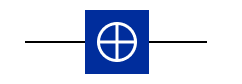
\includegraphics[width=\linewidth]{figures/X-gate.PNG}
    \caption{X-gate}
  \end{subfigure}
  \begin{subfigure}[b]{0.3\linewidth}
    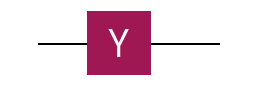
\includegraphics[width=\linewidth]{figures/Y-gate.PNG}
    \caption{Y-gate }
  \end{subfigure}
  \begin{subfigure}[b]{0.3\linewidth}
    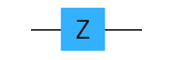
\includegraphics[width=\linewidth]{figures/Z-gate.PNG}
    \caption{Z-gate }
  \end{subfigure}
  \caption{X, Y and Z gate}
  \label{fig:xyzgate}
\end{figure}

X gate on a qubit$\ket{\Psi}$ given by \eqref{eq: 2.1} is
\\$X\ket{\Psi} = X(\alpha\ket{0} + \beta\ket{1}) = \begin{pmatrix}0 &1 \\ 1 &0 \end{pmatrix}\begin{pmatrix}\alpha \\ \beta \end{pmatrix} = \begin{pmatrix}\beta \\ \alpha \end{pmatrix}$

X gate transform $\ket{0}$ to $\ket{1}$ and  transform $\ket{1}$ to $\ket{0}$. It is analogous to the NOT gate in classical computing.\\ 
Hadamard gate(H gate) is another important single-qubit gate in \acrshort{QC}. This gate causes two consecutive rotations on qubit: $90^{\circ}$ about Y-axis followed by $180^{\circ}$ about the X-axis. The Hadamard matrix is
\begin{center}$H = \frac{1}{\sqrt{2}}\begin{pmatrix}1 &1 \\1 &-1\end{pmatrix}  $\end{center}
H gate when acted on a basis state(say $\ket{0}$) produces a superposition of all basis state ($\ket{0}$ and $\ket{1}$):
$H\ket{0} = \frac{\ket{0} +\ket{1}}{\sqrt{2}}$ and $H\ket{1} = \frac{\ket{0} -\ket{1}}{\sqrt{2}}$

\begin{figure}[H]
    \centering
    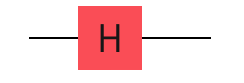
\includegraphics{figures/Hadamard.PNG} 
    \caption{Hadamard Gate }
    \label{fig:hadamard_gate}
\end{figure}

The phase shift gate can be used to manipulate the relative phase of a qubit. Changing the relative phase implies rotating state vector by angle $\phi$ about z-axis with respect to another. For doing that one can either rotate both $\ket{0}$ and $\ket{1}$ by angles $- \phi/2$ and $\phi/2$ respectively or only rotate $\ket{1}$ by angle $\phi$. In doing so, the amplitude of the output state vector is the same as that of the original. The phase shift gate is
\\$R_{\phi}$ = $\begin{pmatrix}1 &0 \\ 0 &e^{i\phi} \end{pmatrix}$ = $e^{i\phi/2}\begin{pmatrix} e^{-i\phi/2} &0 \\ 0 &e^{i\phi/2} \end{pmatrix}$ 
\begin{figure}[H]
    \centering
    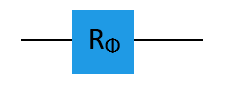
\includegraphics{figures/phasegate.PNG} 
    \caption{Phase-Shift Gate }
    \label{fig: phase_shiftgate}
\end{figure}

When $\phi=\pi$, $R_{\phi} = Z$ gate

\subsection{Multi qubit Gates}
The efficiency of \acrshort{QC} is realized only by the use and association of the multiple numbers of qubits. CNOT, SWAP, CCNOT, C-$R_{\phi}$ are some important multi-qubit gates in \acrshort{QC}. CNOT is a Controlled-NOT gate. A controlled gate is a multi-qubit gate with a set of qubits classified as control qubits and a qubit as a target qubit, such that upon meeting a certain condition in control qubit, an operation is acted upon the target qubit. In other words, control qubits control the state of the target qubit.

A CNOT gate takes two inputs: control bit and target bit. It leaves the target bit unchanged if the control bit is $\ket{0}$ and performs X gate or NOT gate if the control bit is $\ket{1}$. Since it is a two-qubit gate, its matrix is of order $4\times 4$.

CNOT = $\begin{pmatrix} 1 &0 &0 &0 \\ 0 &1 &0 &0 \\ 0 &0 &0 &1 \\ 0 &0 &1 &0 \end{pmatrix}$ 
\begin{figure}[H]
    \centering
    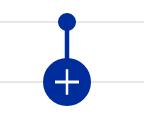
\includegraphics{figures/CNOT.png} 
    \caption{CNOT gate}
    \label{fig:CNOT}
\end{figure}
Mathematically, the transformation is 
\\$CNOT\ket{00} \rightarrow \ket{00}, CNOT\ket{01} \rightarrow \ket{01}, CNOT\ket{10} \rightarrow \ket{11}, CNOT\ket{11} \rightarrow \ket{10}$

CNOT gate is used to create entanglement in \acrshort{QC}. To realize a entangle system let us construct a quantum circuit as shown in fig(\ref{fig: bellstate_plus_circuit}). Before measurement, the qubit $q_{0}$ would be in state $\frac{1}{\sqrt(2)}(\ket{0} + \ket{1}$ ,i.e superposition state. The CNOT gate on the qubits result qubit $q_{1}$ to be in state $\ket{0}$ if the qubit $q_{0}$ is in state$\ket{0}$ or to be in state $\ket{1}$ if the qubit $q_{0}$ is in state $\ket{1}$. Here, just by knowing the state of the qubit $q_{0}$, the state of the qubit $q_{0}$ could be known.\cite{anderzen2018} This represents the entanglement of the two qubits. The final state of the system before measurement is $\frac{1}{\sqrt(2)}(\ket{00} + \ket{11}$. This state is one of the Bell state or EPR pairs. \cite{Nielsen2002}\emph{(Nielsen and Chuang, 2010,p. 25)}

\begin{figure}[H]
  \centering
  \begin{subfigure}[b]{0.3\linewidth}
    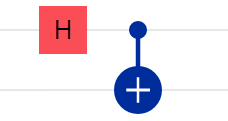
\includegraphics[width=\linewidth]{figures/bellstatecircuit.PNG}
    \caption{Circuit Diagram}
  \end{subfigure}
  \begin{subfigure}[b]{0.3\linewidth}
    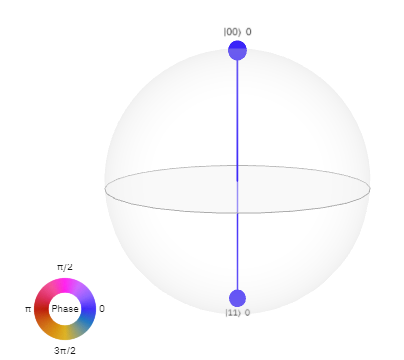
\includegraphics[width=\linewidth]{figures/bellstateqsphere.PNG}
    \caption{Q-sphere for Bell state}
  \end{subfigure}
  \caption{Circuit for Bell state and visualization}
  \label{fig: bellstate_plus_circuit}
\end{figure}

Controlled-U gate can be considered as the generalized version of CNOT gate.\cite{Cheung} Consider U be a $t$ qubit operator and $\ket{\Psi}$ be a quantum register with t qubits as target register and $\ket{q}$ be the control qubit. Controlled-U gate on a system $\ket{q} \ket{\Psi}$ allows the qubit $\ket{q}$ to control the operation $U$ on register $\ket{\Psi}$. That is, the output is $U\ket{\Psi}$ if $\ket{q} = 1$ and the output is $\ket{\Psi}$ if $\ket{q} = \ket{q}$. The circuit diagram for the Controlled-U gate is as shown in figure(\ref{fig: Controlled_U}). 

\begin{figure}[H]
    \centering
    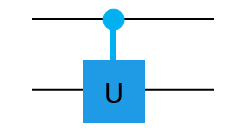
\includegraphics{figures/controlled_U.PNG} 
    \caption{Controlled-U gate}
    \label{fig: Controlled_U}
\end{figure}

After studying the condition of reversibility for quantum gates, one may speculate that irreversible classical logic gates could not be realized in \acrshort{QC}. Fortunately, it was already realized that all the classical gates can be converted into reversible operators, so there's a unitary operator for all the irreversible gates. \cite{Cheung} (Cheung, p10) So it could be generalized that quantum gates are the generalization of the classical gates. An example of this is the realization of the XOR gate by the CNOT gate. CNOT operation on system $\ket{a,b}$ is $$CNOT\ket{a,b} = \ket{a,b \oplus a}$$, where $b \oplus a$ is the XOR operation on $a$ and $b$. The generalized form of conversion of the irreversible circuit into an irreversible one is as follows:
\begin{equation}
		\ket{x,y}
        \begin{cases}
        	\ket{x} \\
            \ket{y \oplus f(x)}
        \end{cases}
\end{equation}

\subsection{Quantum Algorithm}
Quantum Computational approach; use of different properties used in \acrshort{QC} like superposition, entanglement, quantum parallelism\footnote{The property of operators in \acrshort{QC} to operate onto all the superimposed states simultaneously.\cite{neven2012}}, has been used to develop different quantum algorithms that would perform a certain task with superiority than classical approaches. The Quantum Computational approach opens a large prospect to develop other algorithms to solve problems or do tasks, which are difficult to solve classically or to decrease the complicity of the classical algorithm. Different algorithmic paradigms are built under the quantum computing approaches and quantum algorithms are built using the combination of such paradigms. Some of the established quantum algorithmic paradigms are Quantum Fourier transform (QFT), the Grover Operator (GO), the Harrow-Hassidim-Lloyd (HHL) method for linear systems, variational quantum eigenvalue solver (VQE), and direct Hamiltonian simulation (SIM).\cite{coles2018}(Coles, 2018). In this paper, we will be discussing the implementation of the Quantum Fourier transform (QFT) in building different algorithms.

\section{Quantum Fourier Transform}
Quantum Fourier Transform (QFT) is rather a popular quantum algorithmic paradigm that acts as the foundation for several important algorithms including the infamous Shor's algorithm which factors integers in polynomial time, compared to the best classical method performing in sub-exponential time.\cite{lin2014} In \acrshort{QC}, information about the state of the qubit is encoded in magnitude and phase of the system. However, information about magnitude can only be accessed easily and information encoded in phase is directly inaccessible. So information encoded in phase is considered as a part of hidden information stored in the qubit. QFT allows us to retrieve such hidden information stored in-phase and magnitude\cite{johnston2019}. QFT retrieves the information by performing Fourier transform of quantum mechanical amplitudes.\cite{Nielsen2002}\emph{(Nielsen and Chuang, 2010, p216)} So QFT is considered as the quantum equivalent of Discrete Fourier transform.

\subsection{Discrete Fourier Transform}
Discrete Fourier Transform is the discrete form of Fourier transform, specifically designed for computation. DFT takes a set of time-domain discrete points and transforms them into frequency domain points. DFT has a very wide application in classical computers specially signal-processing, data compression, data cleaning, and filtration.

DFT takes a set of N complex numbers: $x_0, x_1, x_2, ...,x_{N-1}$ as input, and transformed them to a another set of N complex numbers: $y_0, y_1, y_2, ...,y_{N-1}$ given by relation:\cite{Nielsen2002}\emph{(Nielsen and Chuang, 2010, p 217)}\begin{equation}
    \centering
    y_k = \frac{1}{\sqrt{N}}\sum_{j=0}^{N-1} e^{2\pi ijk/N}x_{j} = \sum_{j=0}^{N-1} w^{jk} x_{j},
\end{equation}where $w = e^{2\pi i/N}$\\
For all the $y_k$, the transformation becomes $Y = W\cdot X$
\begin{equation}
    \begin{pmatrix}
        y_0\\y_1 \\y_2\\.\\.\\.\\y_{N-1}
    \end{pmatrix}=\frac{1}{\sqrt{N}}
    \begin{pmatrix}
        w^{0} &w^{0} &w^{0} &. &.&. &w^{0}\\
        w^{0} &w^{1} &w^{2} &. &.&. &w^{N-1}\\
        w^{0} &w^{2} &w^{4} &. &.&. &w^{2(N-1)}\\
        . &. &.&.&.&.&.\\
        . &. &.&.&.&.&.\\
        . &. &.&.&.&.&.\\
        w^{0} &w^{N-1} &w^{2(N-1)}  &. &.&. &w^{(N-1)(N-1)}\
    \end{pmatrix}
    \begin{pmatrix}
         x_0\\x_1 \\x_2\\.\\.\\.\\x_{N-1}
    \end{pmatrix}
\end{equation}
It has an algorithmic complexity of $O(n^{2}$. By some clever manipulation using the recursive nature of the problem, an improved version namely \acrlong{FFT}(\acrshort{FFT}) was developed. \acrshort{FFT} is widely used for most practical applications and is considered the best technique for discrete Fourier transform. It has complexity of $O(n \log{n})$.  "The recursive nature of the solution of \acrshort{FFT} sets a stage for studying QFT"\cite{loceff2015} \emph{(Loceff, 2015,p 591)}

\subsection{Quantum Fourier Transform}
Consider a n qubit system given by $\ket{\Psi} = \sum_{k=0}^{N-1} c_{k}\ket{k}$\eqref {eq:2.2} where $N=2^{n}$. Quantum Fourier Transform on the linear combination $\ket{\Psi}$ is a transformation to a another linear combination $\sum_{k=0}^{N-1} d_{k}\ket{j}$ where $j = 0,1,2,...,N-1$ defined by
\begin{equation}
     \ket{j} = \frac{1}{\sqrt{N}}\sum_{k=0}^{N-1} e^{2\pi ijk/N}\ket{k}  = \frac{1}{\sqrt{N}} \sum_{k=0}^{N-1} w^{jk} \ket{k},
\end{equation}where $w = e^{2\pi i/N}$.\\
The transformation is 
\begin{equation}
    \sum_{k=0}^{N-1} d_{k}\ket{j} = \frac{1}{\sqrt{N}} \sum_{k=0}^{N-1} \sum_{j=0}^{N-1} c_k e^{2\pi ijk/N}\ket{k}
\end{equation}\cite{loceff2015}\\
We can see this is a mapping from the vector of N probability amplitude of original system $\ket{\Psi}$ to another vector of new N amplitudes of state for the system. The transformation matrix  for mapping is
\begin{equation}
    W =\frac{1}{\sqrt{N}}
    \begin{pmatrix}
        w^{0} &w^{0} &w^{0} &. &.&. &w^{0}\\
        w^{0} &w^{1} &w^{2} &. &.&. &w^{N-1}\\
        w^{0} &w^{2} &w^{4} &. &.&. &w^{2(N-1)}\\
        . &. &.&.&.&.&.\\
        . &. &.&.&.&.&.\\
        . &. &.&.&.&.&.\\
        w^{0} &w^{N-1} &w^{2(N-1)}  &. &.&. &w^{(N-1)(N-1)}\
    \end{pmatrix}\label{eq:2.9}
\end{equation}
The matrix $W$ is unitary since $W\cdot W^{\dag} = W^{\dag} \cdot W = I$. Hence, QFT circuit is a reversible i.e. is a valid quantum circuit. 

\subsection{Construction of QFT circuit}
We would need to disintegrate the transformation matrix \eqref{eq:2.9} of QFT to the number of individual gates applied to single qubits or multiple qubits for the construction of the circuit.
QFT on  n qubit system with quantum state $\ket{j}$ undergoes transformation  given by \begin{equation}\raggedleft
     \ket{j} \longrightarrow \frac{1}{\sqrt{N}} \sum_{k=0}^{N-1} w^{jk} \ket{k},
\end{equation}where $w = e^{2\pi i/N}$.\\
where $\ket{j} = \ket{j_{1}j_{2} . . . j_{n-1}j_{n}}$ has the binary representation such that $j = 2^{n-1}j_{1} + 2^{n-2}j_{2} + ... + 2^{1}j_{n-1} + 2^{0}j_{n} = \sum_{l=1}^{n} 2^{n-l} j_r$,  $j_{i}\in \{0,1\}$ . Also fraction binary representation $0.j_1j_{l-1} . . . j_{m}$ is given by $ \frac{j_1}{2} + \frac{j_{l+1}}{4} + . . . \frac{j_{m}}{2^{m-l+1}}$\\
So,  \begin{equation}\raggedleft
     \ket{j} = \frac{1}{\sqrt{N}} \sum_{k_1k_2 . . . k_n \in \{0,1\}}^{N-1} w^{j{\sum_{r=1}^n} k_r 2^{n-r}} \ket{k_1k_2k_3 . . . k_n}
\end{equation}
\begin{equation}\raggedleft
      = \frac{1}{\sqrt{N}} \sum_{k_1k_2 . . . k_n \in \{0,1\}}
     \bigotimes_{r=1}^n w^{j k_r 2^{n-r}} \ket{k_r}
\end{equation}
\begin{equation}\raggedleft
      = \frac{1}{\sqrt{N}} \bigotimes_{r=1}^{n} \bigl( \sum_{k_r \in \{0,1\}} w^{j 2^{n-r} k_r} \ket{k_r}\Bigr)
\end{equation}
\begin{equation}\raggedleft
      = \frac{1}{\sqrt{N}} \{\bigotimes_{r=1}^n \bigl( \ket{0} + w^{j 2^{n-r} } \ket{1}\Bigr)\}
\end{equation}
\begin{equation}\raggedleft
      = \frac{1}{\sqrt{N}} \bigotimes_{r=1}^{n} \bigl( \ket{0} + e^\frac{2\pi i 2^{n-r}}{2^n}  \ket{1}\Bigr)
\end{equation}
\begin{equation}\raggedleft
      = \frac{1}{\sqrt{N}} \bigotimes_{r=1}^{n} \bigl( \ket{0} + e^{2\pi i j  2^{-r} } \ket{1}\Bigr)
\end{equation}
\begin{equation}\raggedleft
      = \frac{1}{\sqrt{N}} \bigotimes_{r=1}^{n} \bigl( \ket{0} + e^{2\pi i \sum_{l=1}^{n} 2^{n-l} j_r  2^{-r} } \ket{1}\Bigr) = \frac{1}{\sqrt{N}} \bigotimes_{r=1}^{n} \bigl( \ket{0} + e^{2\pi i \sum_{l=1}^{n} 2^{n-l-r} j_r} \ket{1}\Bigr)
\end{equation}\\
And let $S= \sum_{l=1}^{n} 2^{n-l-r} j_l $
put $r=n$, $S= \sum_{l=1}^{n} 2^{-l} j_r = \frac{j_1}{2} + \frac{j_2}{4} + . . . + \frac{j_n}{2^n} = 0.j_1 j_2 . . . j_n$,\\
put $r=n-1$, $S= \sum_{l=1}^{n} 2^{-(l-1)} j_r = j_1 + \frac{j_2}{2} + \frac{j_3}{4} + . . . + \frac{j_n}{2^{n-1}} = j_1 + 0.j_2 j_3 . . . j_n$\\
Similarly,at $r=1$, $S= \sum_{l=1}^{n} 2^{(n-1)-l} j_r = j_1 + j_2  + j_3 + . . . +j_{n-1} + 0.j_n$\\
But $e^{2\pi i j_1} = e^{2\pi i (j_1 +j_2)} = e^{2\pi i (j_1 + j_2 + . . . j_{n-1})} =1 $\\
So, we could write \begin{equation} 
    \ket{j}  \longrightarrow \frac{1}{\sqrt{N}} \bigl( \ket{0} + e^{2\pi i 0.j_n } \ket{1}\Bigr) \bigl( \ket{0} + e^{2\pi i 0.j_{n-1} j_n } \ket{1}\Bigr) \bigl( \ket{0} + e^{2\pi i 0.j_1 j_2 . . . j_n } \ket{1}\Bigr)
\end{equation}
Now let us use these equations to generate gates, we are familiar with
\begin{enumerate}
 \item The first part of equation $\ket{t_n} = \frac{1}{\sqrt{2}} \bigl( \ket{0} + e^{2\pi i 0.j_n } \ket{1}\Bigr)$ can be realized as a result of applying Hadamard gate on qubit $\ket{j_n}$, 
 that is, if $j_n = 0, \ket{t_n} = \frac{1}{\sqrt{2}} \bigl( \ket{0} + \ket{1} \bigr) = H\ket{0}$
 \\if $j_n = 1, \ket{t_n} = \frac{1}{\sqrt{2}} \bigl( \ket{0} - \ket{1} = H\ket{1}$
 \item The second part $\ket{t_{n-1}} = \frac{1}{\sqrt{N}} \bigl( \ket{0} + e^{2\pi i 0.j_{n-1} j_n } \ket{1}\Bigr)$ can be realized as the result of applying Hadamard gate on $\ket{j_{n-1}}$ followed by controlled phase rotation by $\ket{j_{n-1}}$ on $\ket{j_n}$, $\ket{t_{n-1}} = H_{n-1} \bigr( \ket{0} + e^{2\pi i j_{\frac{n}{4}} \ket{1}} = H_{n-1} R_{\frac{n}{2}} \ket{j_{n-1}}$
 \item Similarly, the other terms can be realized by applying the Hadamard gate followed by a series of controlled phase rotation. So,  $\ket{t_1} = \frac{1}{\sqrt{2}} \bigr( \ket{0} + e^{ 2 \pi i 0.j_1 j_2 . . . j_n} \ket{1}$
\end{enumerate}
The final obtained set of qubits must be reversed for it to match with the equation [2.18]. It is obtained by $\frac{n}{2}$ number of a qubit swap operation. 
The Circuit diagram for generalized QFT is as shown in the figure.

\begin{figure}[H]
    \centering
    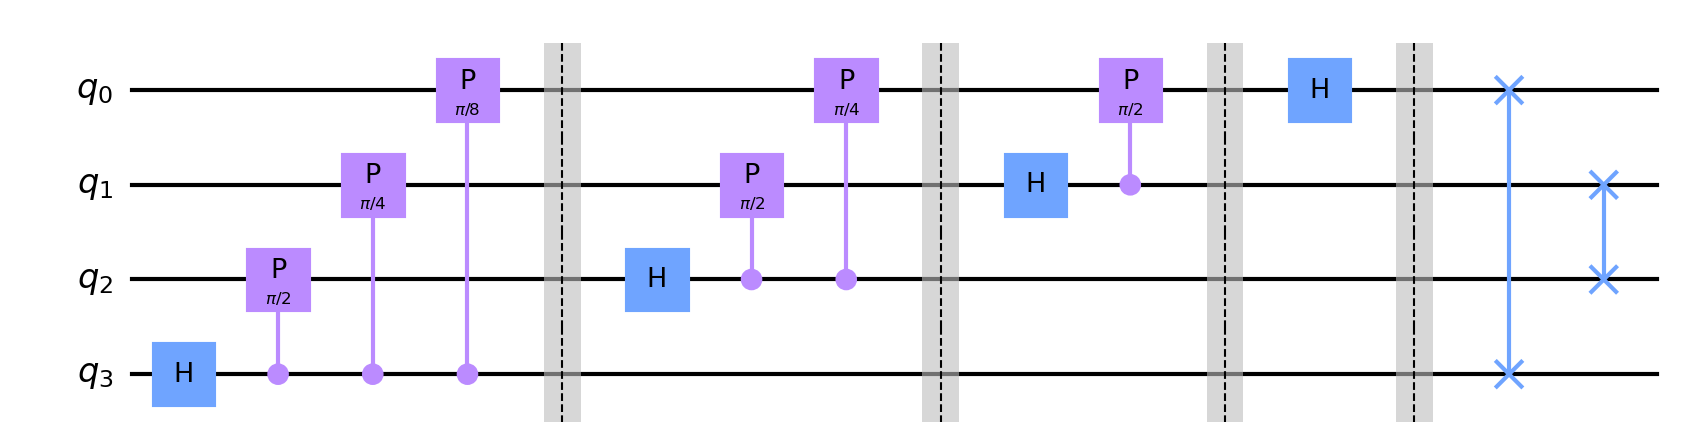
\includegraphics[width = \linewidth]{figures/QFT_for_4q.png}
  \caption{Circuit Diagram of Quantum Fourier transform(\acrshort{QFT}) on a four qubit system}
  \label{fig: QFT circuit diagram}
\end{figure}

\subsubsection{Complexity of QFT}
From the figure, the first line has n gates, the second one has $n-1$, and so on. There are $\sum n = \frac{n\bigr(n-1\bigl)}{2}$ number of gates for QFT transformation and $\frac{n}{2}$ swap gates for further arrangement. Hence the algorithm complexity of the circuit is polynomial. It has $\mathcal{O}\bigr(n^2\bigl)$ complexity.
Comparing with classical \acrshort{FFT} whose complexity is $\mathcal{O}\bigr(n 2^n\bigl)$, QFT seems highly promising. However, there are some major complications that make QFT ineffective for classical \acrshort{FFT} operation. Such complications are errors in measurement of all amplitudes, collapse of superposition upon measurement, and difficulty in creating the initial state.

\subsection{Phase Estimation}
Phase estimation is not a complete algorithm to do a particular task but a subroutine that performs important operation in \acrshort{QC} for determining the information encoded in phase of qubit \cite{johnston2019}. Phase estimation has QFT as its key component during the procedure \cite{Nielsen2002}. Global phases are unobservable by direct measurement. For example, state $\ket{\Psi_1} = \frac{1}{\sqrt{2}}(\ket{0} + e^{i \frac{\pi}{2}} \ket{1})$ and $\ket{\Psi_2} = \frac{1}{\sqrt{2}}(\ket{0} + e^{-i \frac{\pi}{2}} \ket{1})$ gives same result on measurement.

This subroutine takes two registers: first registers of t qubits initialized at state $\ket{0}$ and second $\ket{1}$ which is an eigenvector to a unitary operator $U^\varphi$ and eigenvalue is $e^{2\pi\varphi}$ (where $\varphi$ is unknown). QFT based phase estimation define phase $\varphi$ to be exact integer multiple of $\frac{1}{2^n}$ and is encoded as binary fraction $\varphi$ = $0.x_1 x_2 . . . x_n$ \cite{Nielsen2002}. Phase estimation extract phase information from register $\ket{u}$ and encodes it in the Fourier basis of 1st register. And upon performing inverse Fourier transform such information could be extracted.

The first step for phase estimation is Hadamard operation on 1st register
$\ket{\Psi_1} = \frac{1}{\sqrt{2^t}} \sum_{j=0}^{2^t - 1} \ket{j} \ket{u}$

Circuit proceed by applying a controlled U operation on a second register with U raised to successive power of 2 as shown in the figure(). 


$\ket{\Psi_2} = \frac{1}{\sqrt{2^t}} \sum_{j=0}^{2^t - 1} \ket{j} U \ket{u}$
                 
$= \frac{1}{\sqrt{2^t}} \sum_{j=0}^{2^t - 1} e^{2\pi\varphi} \ket{j} \ket{u}$
                 
We use the information of phase kickback to proceed and perform inverse quantum Fourier transform to get:
$$\ket{\Psi_1} = \ket{\tilde{\varphi_u}} \ket{u}$$
And finally measuring the first register would give the state $\ket{\tilde{\varphi_u}}$ 

The number of qubits in the first register(t) is important in phase estimation as it defines the accuracy and precision of the phase of qubits in register  $\ket{u}$. For example, for 3 qubit 1st register, the circuit could accurately estimate angles $\frac{2\pi }{8} n$ where n = 0, 1, 2, . . 7, as phase of state $\ket{u}$. Similarly, for 4 qubit register, only if $\ket{u}$ is at a phase among one of the angles: $\frac{2\pi }{16} n$ where n= 0, 1, 2, . . . 15, the circuit could accurately find phase.

$\ket{\tilde{\varphi_u}}$ is measured to be one of $R = 2^t$ states. If the measured state is $i \in [0, 2^t -1]$, it suggests the state $\ket{u}$ has angle $\frac{2 \pi i}{n}$.

If the number of a register is not enough i.e. resolution of $\psi$ is not enough, the output ends up in superposition around the closest possible value. One could estimate a low-resolution phase with some probability.

\section{Number theory Background}
Let us introduce some background of the number theory necessary for the study.
\subsection{Modulo Operation}
The reminder $r$ upon dividing a number $b$ by $a$ is output of modular operation: $b$  $mod$  $a$, where $mod$ denotes modular operation. Mathematically, it is represented as :  
\begin{center}
     $b$  mod  $a = r$  or  $b \equiv  r$ (mod $a$) 
\end{center}
Modulo operation is equivalent to division as :
 $b = q*a + r$  where $q$: an integer ($q$ $\in \mathbb{Z}$), is the quotient of division operation of b, dividend by a divisor. 
Some important properties in modular operation are:
\begin{itemize}
    \item (b mod a) mod a = b mod a
    \item $b^x$ mod a = 0 for all x $\in \mathbb{Z} $
    \item ((-b mod a) + (b mod a)) mod a = 0
    \item (b + c) mod a = ((b mod a) + (c mod a)) mod a 
    \item b*c mod a = ((b mod a) (c mod a)) mod a
\end{itemize}
\subsection{Greatest Common Divisor(GCD)}
The greatest common divisor of two integers P and Q denoted by GCD(P, Q) is the largest integer r such that r exactly divides P and Q exactly, i.e. $r$ $\mid$ $P$ and r $\mid$ Q \footnote{a $\mid$ b denotes a divisibility relation such that b is exactly divisible by a or a is a factor of b}.
\begin{definition}
    Two integers $a$ and $b$ are defined as relatively prime to each other, if $GCD(a,b) = 1,$ expressed as $(a \phi b). $
\end{definition}
We use the Euclidean algorithm to find GCD. 
\begin{lemma}
    For $P,Q \in \mathbb{N}: P > Q$ and $ p = q*Q + r$, $ GCD(P,Q) = GCD(Q,r)$ and $ GCD(a,0) = a $
\end{lemma}
\subsubsection{Euclidean Algorithm}
To compute the GCD of integers P and Q : $(P>Q)$, the euclidean algorithm is as follows:
\begin{enumerate}
    \item Initialize $r_0=P$ and $r_1= Q$
    \item Compute $r_2$ such that $r_0 = q_0 * r_1 + r_2$
    \item if $r_2$= 0, $GCD(P,Q) = r_1$
    \item  Since $GCD(r_0,r_1) = GCD(r_1,r_2) $, compute $GCD(r_1,r_2)$. So, put $r_0 = r_1$ and $r_1 = r_2$ and go to step 2
\end{enumerate}

\subsubsection{Time complexity of Euclidean Algorithm}
We have, $ p = q*Q + r$ with  $P > Q > r\in \mathbb{Z} $ \linebreak
If $Q \leq \frac{P}{2}$, then $r < \frac{P}{2}$ since $r < Q$ and if $Q > \frac{P}{2}$, then $r = P - Q \leq \frac{P}{2}$. \linebreak
We can see, the reminder $r_0$ is halved in every two iterations. So, an even $r_2$ becomes 0 with at most $2logP$ iterations. Hence the number of steps is $\mathcal{O}(2logP) = \mathcal{O}(log P)$. Now, each of the steps is division operation and has $\mathcal{O}(log^2 P)$ complexity. Hence the total algorithmic complexity of the Euclidean algorithm is $\mathcal{O}(log^3 X)$ where $X$ is the largest between P and Q.

\subsection{Modular exponentiation function and its order} \label{sbsec: MEF}
A \acrlong{MEF}\acrshort{MEF} is a function in form $f(x) = z^x  $mod$  $n$  $ for $x \in \mathbb{Z}$. It is a periodic function and its period is equal to the order of the function.
\begin{definition}
    Order of  modular function $z^x$ $mod$ $n$ is the smallest integer $x > 1$ such that 
    \begin{center}
         $z^x \equiv$ 1 (mod n)  or  $z^x$ mod n $= 1$
    \end{center}
\end{definition}

$f(x)$ is an injective periodic function.\cite{loceff2015} That means if a is the period, then for every $x \in {0, 1, 2, . . ., a-1}$ maps to distinctly unique element with periodicity at interval of a. i.e. For all $ y \in \{0, 1,,2, . . ., r-1\}$, $f(y) = f(y + a) = f(y + 2a) = . . . = f(y + (m-1)a)$
$\Rightarrow f(y) = f(y + ja) \rfloor_{j=0} ^{m-1} $ where $m = \frac{N}{a}$ is frequency of a.

\begin{figure}[H]
\centering
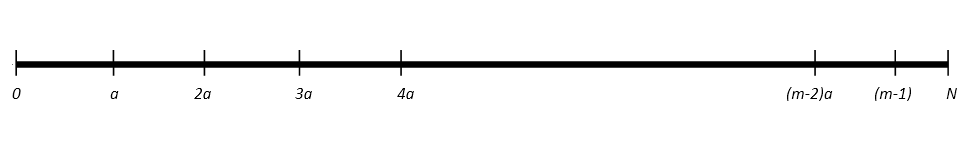
\includegraphics[scale=0.6]{figures/period_line.PNG}
\caption{Line scale showing periodicity of $f(x)$}
\label{fig: Period_a}
\end{figure}
Hence, we can partition the whole input domain: $x \in [0, N-1]= \mathbb{Z}$ into m or m+1 partitions called cosets, where m is the number of the periodicity of the system. We can write,
 \\ $\mathbb{Z} = Q \cup (Q+a) \cup (Q+2a) \cup . . . \cup (Q+(m-1)ma) \cup <Q+ma>$
\\ = $[0,a-1] \cup [a,2a -a] \cup . . . \cup [(m-1)a,ma-1]$
\\ =$\bigcup_{j=0}^{m-1}\{x + ja\}_{x=0}^{N-ma-1}$


Example: (1). Say z= 3, N= 16, $f(x) = 3^x$ (mod 16) \label{lab: Case I}


\begin{table}[h]
\begin{center}
\begin{tabular}{|c|c|c|c|c|c|c|c|c|c|c|c|c|c|c|c|}
\hline
f(0) & f(1) & f(2) & f(3) & f(4) & f(5) & f(6) & f(7) & f(8) & f(9) & f(10) & f(11) & f(12) & f(13) & f(14) & f(15) \\ \hline
1    & 3    & 9    & 11   & 1    & 3    & 9    & 11   & 1    & 3    & 9     & 11    & 1     & 3     & 9     & 11    \\ \hline
\end{tabular}
 \caption{MEF for function $f(x) = 3^x$ mod 16}
 \label{tab: caseI}
 \end{center}
\end{table}

(2). z= 2, N= 15, $f(x) = 2^x$ (mod 15) \label{lab: Case II}
 \begin{table}
\begin{center}
\begin{tabular}{|c|c|c|c|c|c|c|c|c|c|c|c|c|c|c|}
\hline
f(0) & f(1) & f(2) & f(3) & f(4) & f(5) & f(6) & f(7) & f(8) & f(9) & f(10) & f(11) & f(12) & f(13) & f(14) \\ \hline
1    & 2    & 4    & 8    & 1    & 2    & 4    & 8    & 1    & 2    & 4     & 8     & 1     & 2     & 4     \\ \hline
\end{tabular}
  \caption{MEF for function $f(x) = 2^x$ mod 15}
 \label{tab: caseII}
\end{center}
\end{table}

\begin{figure}[H]
  \centering
  \begin{subfigure}[b]{0.4\linewidth}
    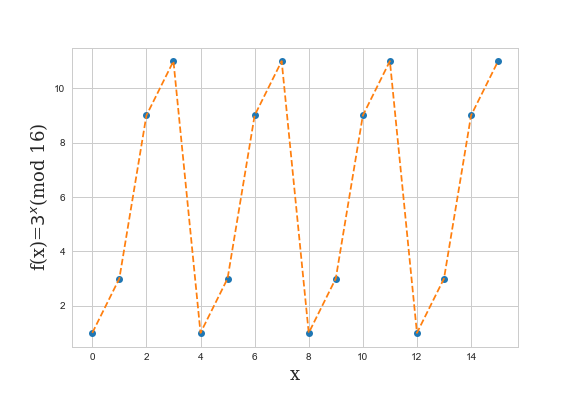
\includegraphics[width=\linewidth]{figures/periodicfunction(3,16).png}
    
    \caption{Output for $f(x)=^x$ (mod 16) }
  \end{subfigure}
  \begin{subfigure}[b]{0.4\linewidth}
    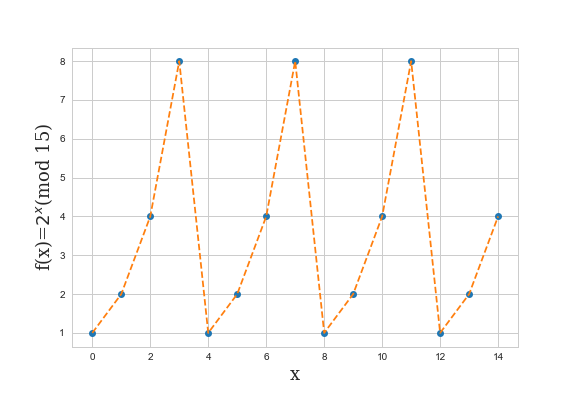
\includegraphics[width=\linewidth]{figures/periodicfunction(2,15).png}
    \caption{Output for $f(x)=2^x$ (mod 15)}
  \end{subfigure}
  \caption{Different cases of periodicity of MEF}
  \label{fig: MEF periodic output graph}
\end{figure}

Example(I) shows the case for m= N which is an ideal case and is impractical for generalization and Example(II) shows the case for $ma \neq N$ which is considered the general case. \par
For easiness in the general case, we define  a number $\tilde{m}$ such that
\\  
$$\tilde{m} = \begin{cases}
    m +1 &\text{ for first few elements in $[0,a-1]$} \\
    m  &\text{ for remaining elements in $[0,a-1]$}
\end{cases}$$

\begin{lemma}
    Suppose $z<N$. z is co-prime with N, then there exist a function $a^{\psi(n)} =1 (mod N)$. \cite{Nielsen2002}(Neilsen et al. 2002,p631)
    \label{th: exist_order_z_N}
\end{lemma}
Lemma \ref{th: exist_order_z_N} states that for two co-primes z<N, the \acrshort{MEF} always has an order 'a'. 

\subsection{Continued Fraction}
A continued fraction is a successive sequence of a fraction of sums and quotients of integer in the form:
\begin{equation*}
   x = a_0+\cfrac{1}{a_1+\cfrac{1}{a_2+\cfrac{1}{ a_3+\cfrac{1}{a_4+\cfrac{1}{a_5+\cdots}}}}}
\end{equation*}
A sequence in form $[a_0:a_1,a_2,a_3,a_4, a_5, \dots ]$ is used to represent the whole object. And the continued fraction sequence is $$\{\frac{n_0}{d_0}, \frac{n_1}{d_1}, \frac{n_2}{d_2}, \frac{n_3}{d_3}, \cdots,\}$$, where 

$\frac{n_0}{d_0} = a_0$, $\frac{n_1}{d_1} = a_0+\cfrac{1}{a_1}$, $\frac{n_2}{d_2} = a_0+\cfrac{1}{a_1+\cfrac{1}{a_2}}$, $\frac{n_3}{d_3} = a_0+\cfrac{1}{a_1+\cfrac{1}{a_2+\cfrac{1}{ a_3}}}$,$\cdots$

Example: $\pi$
\begin{equation*}
    \pi = 3+\cfrac{1}{7+\cfrac{1}{15+\cfrac{1}{1+\cfrac{1}{292+\cdots}}}}
\end{equation*}
With sequence: $\{3,\frac{22}{7}, \frac{333}{106},\frac{355}{115},\frac{103993}{33102}, \cdots \}$

A continued fraction to a finite number of terms is called a finite continued fraction. All rational numbers have a finite continued fraction and irrational numbers have an infinite continued fraction.
\subsubsection{Convergence of continued fraction}
The $k^{th}$ convergent of a continued fraction $[a_0:a_1,a_2,a_3,a_4, a_5, \cdots a_n]$ is 
$C_k = \frac{n_k}{d_k}$ is the $k^{th}$ term in the continued fraction sequence and is the $k^{th}$ approximation of $a_n$.\cite{burton2011}

Some important properties of a continued fraction are
\begin{enumerate}
    \item Every odd index convergents are strictly decreasing and every even index convergents are strictly increasing. 
    \\ Since the convergents eventually converge to a point, every odd index congruent is greater than every even index convergents. 
    \\For a continued fraction of $x$,
    $\frac{n_k}{d_k}$ = $\begin{cases}
                            >x &\text{if k is odd} \\
                            <x &\text{if k is even }
                        \end{cases}$
   \\ It can be visualized using an example and the figure below.
   \begin{equation*}
    \frac{127}{55} = 2+\cfrac{1}{3+\cfrac{1}{4+\cfrac{1}{4}}}
\end{equation*}
and sequence is $\{2,\frac{7}{3}, \frac{30}{13},\frac{127}{55}\}$
    \item The $k^{th}$ convergent $\frac{n_k}{d_k}$ of finite simple continued fraction $x=[a_0:a_1,a_2,a_3,a_4,\cdots ]$ follows:
    $\mid \frac{n_k}{d_k} - \frac{n_{k-1}}{d_{k-1}}\mid = \frac{1}{d_k d_{k-1}}$
    
    \item For all the convergents $\frac{n_k}{d_k}$ in a finite continued fraction sequence of $x=d_K$, the denominator is strictly increasing.i.e. $d_k > d_{k-1}$ for all $0<k<K$ 
\end{enumerate}

\subsubsection{Approximation}
\begin{definition}
    An convergent $\frac{n_k}{d_k}$ of continued fraction of x is said to be an good approximation of x, if $\frac{n_i}{d_i} \neq \frac{n_k}{d_k}$ and ${d_i} < {d_k}$ for all $0<i<k$.\cite{raji2013}
    \begin{equation*}
        \abs{ x - \frac{n_k}{d_k}} < \abs{x - \frac{n_i}{d_i}} 
    \end{equation*} for all $0<i<k$

\end{definition}
It means $\frac{n_k}{d_k}$ is closest to x than all other convergent with denominator less than $d_k$.

\begin{lemma}
    "Let x be an real number. If the rational number $\frac{n}{d}$, where $d \geq 1$ and $GCD(n,d)=1$, satisfies 
    \begin{equation}
        \abs{x- \frac{n}{d}} < \frac{1}{2d^2}
    \end{equation}
    ,then $\frac{n}{d}$ is one of the convergents $\frac{n_k}{d_k}$ in the continued fraction sequence of x." \cite{burton2011}(Burton, 2011)
    \label{th: approx_cont_frac}
\end{lemma}
% \begin{proof}
%     is needed???
% \end{proof}



\subsubsection{Continued fraction Algorithm}

\begin{algorithm}[H]
  \KwData{A number: num, error:E}
  \KwResult{Convergent: $\frac{n_k}{d_k}$}
  Initialization: Input number=num, Error= E \;
  Compute $a_0 = \lfloor num \rfloor$\;
  \uIf{$(\frac{num}{a_0} \neq 1)$}{
    Compute $a = \lfloor \frac{1}{num-a_0} \rfloor$\;
    Compute $n_0= a_0; d_0=1$ \;
    Compute $n_k=n_1= a*a_0 + 1; d_k=d_1= a$ \;
    \While{($\abs{\frac{n_k}{d_k} - num} \geq E$)}{
         Compute $a = \lfloor \frac{1}{num-a} \rfloor$;\;
         Compute $n_k= a*n_1 + n_0$, $d_k= a*d_1 + d_0$\;
         Set $n_0 =n_1,$ $ d_0 = d_1$\;
         Set $n_1 =n_k,$ $ d_1 = d_k$\;
     }
    {Output: $\frac{n_k}{d_k}$\;}
  }
  \Else{
        Output: num\;} 
  \caption{Algorithm to output a approximate convergents of a continued fraction bounded by an error}
  \label{algo: Continued_fraction_Alorithm}
\end{algorithm}

\section{Complexity}
Computational complexity is the study of problem analysis to categorize them based on resources like time, space, and energy required to solve the problem.\cite{Nielsen2002} One can speculate that a search algorithm is harder and require more resources than an addition algorithm. Different problems may require a different amount of resources. Even for a single problem, different algorithms, requiring different amounts of time or space, can be used to determine the same output. The algorithm is the set of steps performing mathematical operations to solve problems. So, they are independent of the hardware used or software implemented. This makes computational complexity a general way to study problems and define efficiency.

The complexity of a problem or algorithm is defined based on the size of the input: bit-length or number of input data, n. It studies how a problem grows as the size of input increases. Conventionally, we use Big $\mathcal{O}$ notation and Big $\Omega$ notation to define complexity. Big $\mathcal{O}$ is used to express the upper-bound of the worst-case during the execution of an algorithm. And Big $\Omega$ represents the lower-bound of the worst case. We will be using Big $\mathcal{O}$ notation more often than Big $\Omega$ in the study. An algorithm has the complexity of $\mathcal{O}(g(n))$ where $g(n)$ is a function of the size of input or number of steps n, which means the algorithm will at most use $g(n)$ amount of space(memory) or take $g(n)$ number of steps to complete. An important property of Big $\mathcal{O}$ notation is that an algorithm is as good as its worst sub-operation or sub-routine. That is, if $f(n)$ is the resources used in an algorithm defined as $f(n)= a_0n^k + a_1n^{k-1}+ \cdot + a_k$, then f is $\mathcal{O}(n^k)$.

Complexity is categorized into subcategories according to the resources used. Time complexity and Space complexity are widely used to measure the efficiency of an algorithm. Time complexity is the study of an algorithm based on the number of steps or time taken to complete. Space complexity deals with the memory or space needed to store data during the execution of the algorithm.
 
In classical computing, there are different complexity classes based on space and time complexity. Figure(\ref{fig: Complexity classesI}) shows various complexity classes with increasing complexity with an increase in the area of the region of the class. Some common and significant complexity classes are:
\begin{figure}[H]
    \centering
    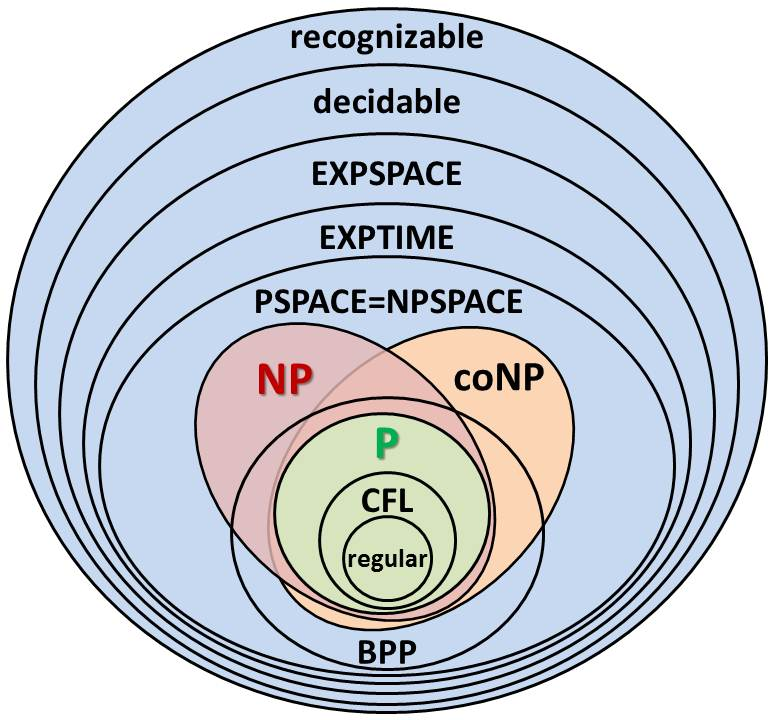
\includegraphics[scale=0.4]{figures/Complexity-classes-diagram.jpg}
    \caption{Some common complexity classes with their relations \protect\cite{complex_classesI}}
    \label{fig: Complexity classesI}
\end{figure}
 
\begin{enumerate}
    \item P class
    \\ P – polynomial class problems are the problems that have polynomial time complexity. This class includes problems with constant $\mathcal{O}(1)$, linear $\mathcal{O}(n)$, logarithmic $\mathcal{O}(log(n))$, log normal $\mathcal{O}(nlog(n))$ and quadratic $\mathcal{O}(n^2)$ and other polynomial complexity
     
    \item NP class
    \\ NP – Non-polynomial class problem has non-polynomial time complexity. The problem in this class has solutions verifiable in polynomial time. However, finding the solution takes non-polynomial time like exponential time.
     
    \item PSPACE
    \\ PSPACE – Polynomial space problem consumes memory in polynomial scale as the input size grows. Figure (\ref{fig: Complexity classesI}) shows the hierarchical position of complexity.
     
    \item BPP
    \\ BPP – Bounded-error probabilistic polynomial class problem is a different type of problem that has a bounded probability of being solved in polynomial time. Polynomial class problem problems are included in it. Usually, problems with a success probability of more than 2/3 are included in this class
     
    \item \acrshort{BQP}
    \\ \acrshort{BQP} - Bounded-error Quantum polynomial problems are similar to BPP problems, except that these problems are solved by quantum computer or quantum algorithm. It covers some problems of NP class and P class problems. The success of an algorithm of this class is bounded by some high probability. We will prove Shor’s algorithm is a \acrshort{BQP} algorithm later in the study.
\end{enumerate}
\begin{figure}[H]
    \centering
    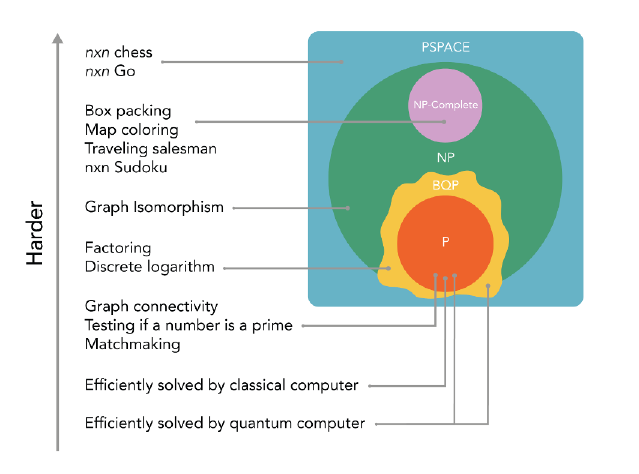
\includegraphics[scale=0.6]{figures/complexity-classes-example.PNG}
    \caption{Figure showing some common complexity classes with their examples \protect \cite{Hidary}(Hidary, 2019, p41)}
    \label{fig: Complexity classesII}
\end{figure}
 